%\documentclass[hyperref={pdfpagelabels=false},slidetop,9pt]{beamer}
\documentclass[slidetop,8pt]{beamer}
\usepackage[T1]{fontenc}
\usepackage[utf8]{inputenc}
\newcommand{\id}{54}
\newcommand{\nom}{Liaisons mécaniques}
\newcommand{\sequence}{04}
\newcommand{\num}{01}
\newcommand{\type}{TP}
\newcommand{\descrip}{Modélisation d'un solide. Comportement des liaisons mécaniques. Modéliser les mécanismes du laboratoire par un schéma cinématique, paramétré.}
\newcommand{\competences}{A3-C4: Analyse d'architecture et de comportement \\ &  Mod1-C1: Isolement d'un solide ou d'un système de solides \\ &  Mod2-C10-1: Modèle de solide indéformable \\ &  Mod2-C11: Modélisation géométrique et cinématique des mouvements entre solides indéformables \\ &  Mod2-C12: Modélisation cinématique des liaisons entre solides \\ &  Mod2-C15: Modélisation des actions mécaniques \\ &  Rés-C6: Utilisation d'un solveur ou d'un logiciel multi physique \\ &  Com1-C1: Différents descripteurs introduits dans le programme \\ &  Com2-C4: Outils de communication}
\newcommand{\nbcomp}{9}
\newcommand{\systemes}{Plateforme Stewart}
\newcommand{\systemessansaccent}{Plateforme Stewart}
\newcommand{\ilot}{2}
\newcommand{\ilotstr}{02}
\newcommand{\dossierilot}{\detokenize{Ilot_02 Plateforme Stewart}}
\newcommand{\imageun}{Plateforme}

\newcommand{\urlsysteme}{\href{https://www.costadoat.fr/systeme/57}{Ressources système}}
\newcommand{\matlabsimscape}{\href{https://github.com/Costadoat/Sciences-Ingenieur/raw/master/Systemes/Plateforme Stewart/Plateforme_Stewart_Simscape.zip}{Modèle Simscape}}
\newcommand{\solidworks}{\href{https://github.com/Costadoat/Sciences-Ingenieur/raw/master/Systemes/Plateforme Stewart/Plateforme_Stewart_Solidworks.zip}{Modèle Solidworks}}
\newcommand{\edrawings}{\href{https://github.com/Costadoat/Sciences-Ingenieur/raw/master/Systemes/Plateforme Stewart/Plateforme_Stewart.EASM}{Modèle eDrawings}}
\newcommand{\test}{Stewart_param1}
\newcommand{\testi}{Stewart_param2}
\newcommand{\testii}{Stewart_param3}
\newcommand{\testiii}{Stewart_param4}
\newcommand{\testiiii}{Stewart_euler}
\usepackage{etex}
\usepackage{tikz}
\usepackage[european]{circuitikz}
\usepackage{pgf}
\usepackage[all]{xy}
\usepackage{pgfpages}
\usepackage{graphbox}
\usepackage{pdfpages}
\usepackage[adobe-utopia]{mathdesign}
\usepackage{ifthen}
\usepackage{cancel}
\usepackage{framed}
\usepackage{subfig}
\usepackage{tabularx}
\usepackage{setspace}
\usepackage{soul}
\usepackage{schemabloc}
\usepackage{eqnarray}
\usepackage[dot, phantomtext]{dashundergaps}
\usepackage{media9}
\usepackage{multimedia}
\usepackage{textcomp}

\author{Renaud Costadoat}
\institute{Lycée Dorian}

\usepackage{multido}
\usepackage{multirow}
\usepackage{multicol} % Portions de texte en colonnes
\usepackage{flafter}%floatants après la référence

\usepackage{color}
\usepackage{xcolor}
\usepackage{colortbl}

\usepackage[gen]{eurosym}
\usepackage{tikz}
%\usepackage{pstricks,pst-node,pst-tree,pst-solides3d}
\usepackage{lmodern}
\usepackage[francais]{babel}
\usepackage{pslatex}
\usetheme{renaud}
\usepackage{times}
\usepackage{amsmath}
\usepackage{verbatim}
\usepackage{moreverb}
%\usetikzlibrary{arrows,shapes}
\usepackage{graphicx}
\usepackage{psfrag}
\usepackage{wrapfig}
\usepackage{etoolbox}

\definecolor{gris25}{gray}{0.75}
\definecolor{bleu}{RGB}{18,33,98}
\definecolor{bleuf}{RGB}{42,94,171}
\definecolor{bleuc}{RGB}{231,239,247}
\definecolor{rougef}{RGB}{185,18,27}
\definecolor{rougec}{RGB}{255,188,204}%255,230,231
\definecolor{vertf}{RGB}{103,126,82}
\definecolor{vertc}{RGB}{220,255,191}

\setlength\parindent{24pt}
\parskip 7.2pt
\parindent 8pt

\newenvironment{rem}[1][\hsize]%
{%
    \def\FrameCommand
   {%
\rotatebox{90}{\textit{\textsf{Remarque}}} 
       {\color{bleuf}\vrule width 3pt}%
       \hspace{0pt}%must no space.
       \fboxsep=\FrameSep\colorbox{bleuc}%
  }%
    \MakeFramed{\hsize#1\advance\hsize-\width\FrameRestore}%
}%
{\endMakeFramed}%


\newenvironment{savoir}[1][\hsize]%
{%
    \def\FrameCommand
    {%
\rotatebox{90}{\textit{\textsf{Savoir}}} 
        {\color{bleuf}\vrule width 3pt}%
        \hspace{0pt}%must no space.
        \fboxsep=\FrameSep\colorbox{bleuc}%
    }%
    \MakeFramed{\hsize#1\advance\hsize-\width\FrameRestore}%
}%
{\endMakeFramed}%

\newenvironment{prob}[1][\hsize]%
{%
    \def\FrameCommand%
    {%
\rotatebox{90}{\textit{\textsf{Problematique}}} 
        {\color{rougef}\vrule width 3pt}%
        \hspace{0pt}%must no space.
        \fboxsep=\FrameSep\colorbox{rougec}%
    }%
    \MakeFramed{\hsize#1\advance\hsize-\width\FrameRestore}%
}%
{\endMakeFramed}%

\newenvironment{obj}[1][\hsize]%
{%
    \def\FrameCommand%
    {%
\rotatebox{90}{\textit{\textsf{Objectif}}} 
        {\color{vertf}\vrule width 3pt}%
        \hspace{0pt}%must no space.
        \fboxsep=\FrameSep\colorbox{vertc}%
    }%
    \MakeFramed{\hsize#1\advance\hsize-\width\FrameRestore}%
}%
{\endMakeFramed}%

\newenvironment{defi}[1][\hsize]%
{%
    \def\FrameCommand%
    {%
\rotatebox{90}{\textit{\textsf{Definition}}} 
        {\color{bleuf}\vrule width 3pt}%
        \hspace{0pt}%must no space.
        \fboxsep=\FrameSep\colorbox{rougec}%
    }%
    \MakeFramed{\hsize#1\advance\hsize-\width\FrameRestore}%
}%
{\endMakeFramed}%


\newenvironment{hypo}[1][\hsize]%
{%
    \def\FrameCommand%
    {%
\rotatebox{90}{\textit{\textsf{Hypothèse\\}}} 
        {\color{bleuf}\vrule width 3pt}%
        \hspace{0pt}%must no space.
        \fboxsep=\FrameSep\colorbox{bleuc}%
    }%
    \MakeFramed{\hsize#1\advance\hsize-\width\FrameRestore}%
}%
{\endMakeFramed}%


\newenvironment{prop}[1][\hsize]%
{%
    \def\FrameCommand%
    {%
\rotatebox{90}{\textit{\textsf{Propriété}}} 
        {\color{bleuf}\vrule width 3pt}%
        \hspace{0pt}%must no space.
        \fboxsep=\FrameSep\colorbox{bleuc}%
    }%
    \MakeFramed{\hsize#1\advance\hsize-\width\FrameRestore}%
}%
{\endMakeFramed}%

\newenvironment{props}[1][\hsize]%
{%
    \def\FrameCommand%
    {%
\rotatebox{90}{\textit{\textsf{Propriétés}}} 
        {\color{bleuf}\vrule width 3pt}%
        \hspace{0pt}%must no space.
        \fboxsep=\FrameSep\colorbox{bleuc}%
    }%
    \MakeFramed{\hsize#1\advance\hsize-\width\FrameRestore}%
}%
{\endMakeFramed}%

\newenvironment{exemple}[1][\hsize]%
{%
    \def\FrameCommand%
    {%
\rotatebox{90}{\textit{\textsf{Exemple}}} 
        {\color{vertf}\vrule width 3pt}%
        \hspace{0pt}%must no space.
        \fboxsep=\FrameSep\colorbox{vertc}%
    }%
    \MakeFramed{\hsize#1\advance\hsize-\width\FrameRestore}%
}%
{\endMakeFramed}%

\newenvironment{resultat}[1][\hsize]%
{%
    \def\FrameCommand%
    {%
\rotatebox{90}{\textit{\textsf{Résultat}}} 
        {\color{rougef}\vrule width 3pt}%
%        {\color{bleuf}\vrule width 3pt}%
        \hspace{0pt}%must no space.
        \fboxsep=\FrameSep\colorbox{rougec}%
    }%
    \MakeFramed{\hsize#1\advance\hsize-\width\FrameRestore}%
}%
{\endMakeFramed}%

\newenvironment{methode}[1][\hsize]%
{%
    \def\FrameCommand%
    {%
\rotatebox{90}{\textit{\textsf{Méthode\\}}} 
        {\color{rougef}\vrule width 3pt}%
        \hspace{0pt}%must no space.
        \fboxsep=\FrameSep\colorbox{rougec}%
    }%
    \MakeFramed{\hsize#1\advance\hsize-\width\FrameRestore}%
}%
{\endMakeFramed}%

\newenvironment{theo}[1][\hsize]%
{%
    \def\FrameCommand%
    {%
\rotatebox{90}{\textit{\textsf{Théorème\\}}} 
        {\color{rougef}\vrule width 3pt}%
        \hspace{0pt}%must no space.
        \fboxsep=\FrameSep\colorbox{rougec}%
    }%
    \MakeFramed{\hsize#1\advance\hsize-\width\FrameRestore}%
}%
{\endMakeFramed}%

\newenvironment{warn}[1][\hsize]%
{%
    \def\FrameCommand%
    {%
\rotatebox{90}{\textit{\textsf{Attention\\}}} 
        {\color{rougef}\vrule width 3pt}%
        \hspace{0pt}%must no space.
        \fboxsep=\FrameSep\colorbox{rougec}%
    }%
    \MakeFramed{\hsize#1\advance\hsize-\width\FrameRestore}%
}%
{\endMakeFramed}%

% \usepackage{pstricks}
%\usepackage{minitoc}
% \setcounter{minitocdepth}{4}

\setcounter{tocdepth}{2}

% \mtcselectlanguage{french} 

%\usepackage{draftcopy}% "Brouillon"
% \usepackage{floatflt}
\usepackage{psfrag}
%\usepackage{listings} % Permet d'insérer du code de programmation
\renewcommand{\baselinestretch}{1.2}

% Changer la num�rotation des figures :
% ------------------------------------
% \makeatletter
% \renewcommand{\thefigure}{\ifnum \c@section>\z@ \thesection.\fi
%  \@arabic\c@figure}
% \@addtoreset{figure}{section}
% \makeatother
 


%%%%%%%%%%%%
% Définition des vecteurs %
%%%%%%%%%%%%
 \newcommand{\vect}[1]{\overrightarrow{#1}}

%%%%%%%%%%%%
% Définition des torseusr %
%%%%%%%%%%%%

 \newcommand{\torseur}[1]{%
\left\{{#1}\right\}
}

\newcommand{\torseurcin}[3]{%
\left\{\mathcal{#1} \left(#2/#3 \right) \right\}
}

\newcommand{\torseurstat}[3]{%
\left\{\mathcal{#1} \left(#2\rightarrow #3 \right) \right\}
}

 \newcommand{\torseurc}[8]{%
%\left\{#1 \right\}=
\left\{
{#1}
\right\}
 = 
\left\{%
\begin{array}{cc}%
{#2} & {#5}\\%
{#3} & {#6}\\%
{#4} & {#7}\\%
\end{array}%
\right\}_{#8}%
}

 \newcommand{\torseurcol}[7]{
\left\{%
\begin{array}{cc}%
{#1} & {#4}\\%
{#2} & {#5}\\%
{#3} & {#6}\\%
\end{array}%
\right\}_{#7}%
}

 \newcommand{\torseurl}[3]{%
%\left\{\mathcal{#1}\right\}_{#2}=%
\left\{%
\begin{array}{l}%
{#1} \\%
{#2} %
\end{array}%
\right\}_{#3}%
}

 \newcommand{\vectv}[3]{%
\vect{V\left( {#1} \in {#2}/{#3}\right)}
}


\newcommand{\vectf}[2]{%
\vect{R\left( {#1} \rightarrow {#2}\right)}
}

\newcommand{\vectm}[3]{%
\vect{\mathcal{M}\left( {#1}, {#2} \rightarrow {#3}\right)}
}


 \newcommand{\vectg}[3]{%
\vect{\Gamma \left( {#1} \in {#2}/{#3}\right)}
}

 \newcommand{\vecto}[2]{%
\vect{\Omega\left( {#1}/{#2}\right)}
}

\newcommand{\reponse}[1][4]
{
\multido{}{#1}
{
\begin{center}
\makebox[0.9\linewidth]{\dotfill} \end{center}
}}


% }$$\left\{\mathcal{#1} \right\}_{#2} =%
% \left\{%
% \begin{array}{c}%
%  #3 \\%
%  #4 %
% \end{array}%
% \right\}_{#5}}


%  ------------------------------------------
% | Modification du formatage des sections : | 
%  ------------------------------------------

% Grands titres :
% ---------------

\newcommand{\titre}[1]{%
\begin{center}
      \bigskip
      \rule{\textwidth}{1pt}
      \par\vspace{0.1cm}
      
      \textbf{\large #1}
      \par\rule{\textwidth}{1pt}
    \end{center}
    \bigskip
  }

% Supprime le numéro du chapitre dans la numérotation des sections:
% -----------------------------------------------------------------
\makeatletter
\renewcommand{\thesection}{\@arabic\c@section}
\makeatother


% \titleformat{\chapter}[display]
% {\normalfont\Large\filcenter}
% {}
% {1pc}
% {\titlerule[1pt]
%   \vspace{1pc}%
%   \Huge}[\vspace{1ex}%
% \titlerule]


%%%% Chapitres Comme PY Pechard %%%%%%%%%
% numéro du chapitre
\DeclareFixedFont{\chapnumfont}{OT1}{phv}{b}{n}{80pt}
% pour le mot " Chapitre "
\DeclareFixedFont{\chapchapfont}{OT1}{phv}{m}{it}{40pt}
% pour le titre
\DeclareFixedFont{\chaptitfont}{T1}{phv}{b}{n}{25pt}

\definecolor{gris}{gray}{0.75}
\setbeamertemplate{section in toc}[sections numbered]

\newlength{\RoundedBoxWidth}
\newsavebox{\GrayRoundedBox}
\newenvironment{GrayBox}[1][\dimexpr\textwidth-4.5ex]%
   {\setlength{\RoundedBoxWidth}{\dimexpr#1}
    \begin{lrbox}{\GrayRoundedBox}
       \begin{minipage}{\RoundedBoxWidth}}%
   {   \end{minipage}
    \end{lrbox}
    \begin{center}
    \begin{tikzpicture}%
       \draw node[draw=bleuf,fill=bleuc,rounded corners,%
             inner sep=2ex,text width=\RoundedBoxWidth]%
             {\usebox{\GrayRoundedBox}};
    \end{tikzpicture}
    \end{center}}
    
\ifdef{\prive}{\pgfpagesuselayout{2 on 1}[a4paper,border shrink=0mm]}
\ifdef{\prive}{\setbeamertemplate{navigation symbols}{}}
\setbeamertemplate{itemize item}[ball]
%\setbeamertemplate{blocks}[rounded]%[shadow=true]
\setbeamercolor{block title}{fg=white,bg=grisf}        % titre block normal 
\setbeamercolor{block body}{fg=grisf,bg=grisc!50}      % corps block normal
\setbeamercolor{block body alerted}{fg=white,bg=warning}   % idem pour un block alerte

\title{\nom}
\date{S\sequence \ - \type\num}

\begin{document}
\shorthandoff{:!}
\bibliographystyle{abbrvnat-fr}

\usebackgroundtemplate%
{%
    \centering
\includegraphics[width=\paperwidth]{../../img/fond2}%
}

{
\setbeamertemplate{navigation symbols}{}
\setbeamertemplate{headline}[pagetitre]
\setbeamertemplate{footline}[pagetitre]
\usebackgroundtemplate{\centering
\includegraphics[width=\paperwidth]{../../img/fond}}
\frame{\titlepage}
}




\section{Transmission de données}

{\frame{
\frametitle{Introduction}

\begin{savoir}
Vous êtes capables :
\begin{itemize}
 \item de caractériser les différents \textbf{cas d'utilisation} d'un produit,
 \item de décrire la \textbf{séquence} de communication entre un \og acteur \fg du système et le système. 
\end{itemize}
\end{savoir}

\begin{prob}
Vous devez êtes capables :
\begin{itemize}
 \item de déduire le comportement séquentiel d'un système à partir des diagrammes dédiés,
 \item de connaître les moyens de mise en \oe uvre de cette programmation.
\end{itemize}
\end{prob}
}}

{\frame{
\frametitle{Types de données}

\begin{center}
 \begin{tabular}{|c|c|c|}
 \hline
 & Transmission analogique & Transmission numérique \\  
 \hline
 Information analogique & ----- (1) & CoDec (4) \\ 
 \hline
 Information numérique & MoDem (3) & ----- (2) \\
 \hline
  \end{tabular}
\end{center}

\begin{enumerate}
 \item Réseau téléphonique analogique,
 \item Ordinateur et périphériques,
 \item Connexion de terminaux distants à un ordinateur central,
 \item Numérisation du réseau téléphonique.
\end{enumerate}
}}

{\frame{
\frametitle{Signaux analogiques/numériques}

Une grandeur est dite:
\begin{itemize}
 \item analogique si sa mesure donne un nombre réel variant de
façon continue. Il existe une infinité de valeurs pour une grandeur
analogique.
 \item numérique si elle est contrainte à ne prendre qu'un
nombres restreints de valeurs. 
\end{itemize}

\begin{minipage}[t]{0.48\linewidth}
Signaux \textbf{analogiques}
\begin{itemize}
 \item représentés par une
grandeur physique variant
de manière continue
\end{itemize}
\centering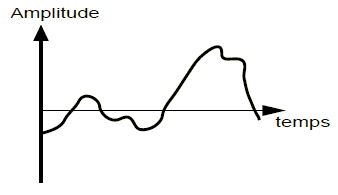
\includegraphics[width=0.8\linewidth]{img/analogique}
\end{minipage}
\begin{minipage}[t]{0.48\linewidth}
Signaux \textbf{numériques}
\begin{itemize}
 \item Représentés par une grandeur
physique de prenant qu'un
certains nombre de valeurs
discrètes.
\end{itemize}
\centering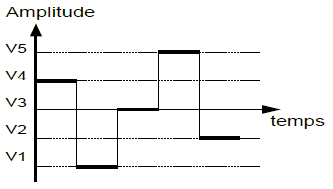
\includegraphics[width=0.8\linewidth]{img/numerique}
\end{minipage}
}}

{\frame{
\frametitle{Numérisation}

\begin{itemize}
 \item Théorème de Nyquist-Shannon:
 \begin{itemize}
  \item Un signal à spectre limité à la bande $-\dfrac{F}{2}$, $+\dfrac{F}{2}$ ($0$, $\dfrac{F}{2}$ dans la pratique) est complètement déterminé par les valeurs échantillonnées à des instant uniformément répartis dans le
temps et égaux à $\dfrac{1}{F}$,
  \item la fréquence d'échantillonage doit être au minimum
égale au double de la fréquence maximale du signal à
échantillonner.
 \end{itemize}
 \item Ce problème intervient aussi lors de calculs numériques (Scilab).
\end{itemize}

Exemples:
\begin{itemize}
 \item Canal téléphonique :
  \begin{itemize}
   \item plage de fréquences : $4000Hz$ ( en fait $300-3400Hz$),
   \item $Fe=4000\times 2=8000Hz$ (1 échantillon toutes les $125\mu s$).
  \end{itemize}
 \item CD audio :
  \begin{itemize}
   \item Plage de fréquence : $20kHz$,
   \item $Fe=20\times 2=40kHz$ (normalisé à $44,1kHz$).
  \end{itemize}
\end{itemize}
}}

{\frame{
\frametitle{Quantification}

\begin{itemize}
 \item Mesure des échantillons à l'aide d'un nombre fini de valeurs.  Numérisation des échantillons,
 \item Passage du continu au discret sur l'axe des ordonnées.
Mesure de l'amplitude du signal avec un nombre fini de
valeurs.
 \begin{itemize}
  \item Approximation à la valeur discrète possible la plus proche (erreur (ou bruit) de quantification),
  \item Compression logarithme pour obtenir un bruit de quantification relatif constant.
 \end{itemize}
\end{itemize}

}}

{\frame{
\frametitle{Codage}

$8$ bits par échantillon en codage MIC (256 valeurs): \\ débit binaire=$8000\times 8=64000bit/s=64kbit/s$.

\begin{center}
 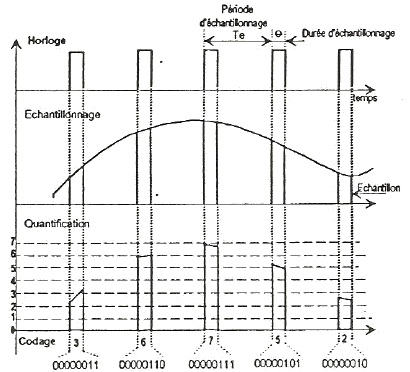
\includegraphics[width=0.6\linewidth]{img/codage}
\end{center}
}}

{\frame{
\frametitle{Mode de transmission}

\textbf{Transmission synchrone}

\begin{center}
 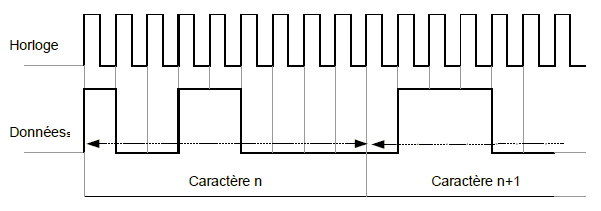
\includegraphics[width=0.8\linewidth]{img/synchrone}
\end{center}

\begin{itemize}
 \item Synchronisation-bit,
 \item Synchronisation-caractère.
\end{itemize}
}}

{\frame{
\frametitle{Mode de transmission}

\textbf{Transmission asynchrone: 50 bauds}

\begin{center}
 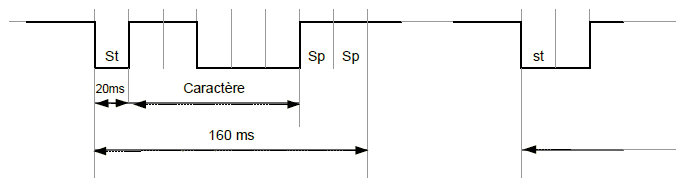
\includegraphics[width=0.8\linewidth]{img/asynchrone}
\end{center}

\begin{itemize}
 \item Nécessité de reconnaître le début et la fin de chaque caractère,
 \item Pas de synchronisation entre 2 caractères.
\end{itemize}
}}

\section{Les types de réseaux}

{\frame{
\frametitle{Les différents types de réseaux}

\begin{itemize}
 \item On distingue différents types de réseaux (privés) selon leur taille (en terme de nombre de machines), leur vitesse de transfert des données ainsi que leur étendue.
 \item On fait généralement trois catégories de réseaux :
 \begin{itemize}
  \item LAN (Local Area Network),
  \item MAN (Metropolitan Area Network),
  \item WAN (Wide Area Network).
 \end{itemize}
 \item Il existe deux autres types de réseaux :
 \begin{itemize}
  \item TAN (Tiny Area Network) identique au LAN mais moins étendus (2 à 3 machines).
  \item CAN (Campus Area Network) identiques au MAN (avec une bande passante maximale entre tous les LAN du réseau).
 \end{itemize}
\end{itemize}
}}	

{\frame{
\frametitle{Le réseau local LAN}

Le réseau local LAN (Local Area Network) en français \og Réseau Local \fg est un réseau informatique à une échelle géographique relativement restreinte. Il est utilisé pour relier entre eux les ordinateurs : par exemple d'une habitation particulière, d'une entreprise, d'une salle informatique, d'un bâtiment. L'infrastructure est privée et est gérée localement.

À l'intérieur, ou « sur » le réseau local il y a des ordinateurs fixes ou portables connectés par des câbles ou sans fil (Réseaux locaux sans fil : WLAN). Ces deux mondes communiquent par l'intermédiaire d'une box ou modem ADSL (selon le FAI).
}}

{\frame{
\frametitle{Le réseau local LAN}

La taille d'un réseau local peut atteindre jusqu'à 100 voire 1000 utilisateurs. En élargissant le contexte de la définition aux services qu'apportent le réseau local, il est possible de distinguer deux modes de fonctionnement :
\begin{itemize}
 \item dans un environnement « paire à paire : P2P » (en anglais peer to peer), dans lequel il n'y a pas d'ordinateur central et chaque ordinateur a un rôle similaire,
 \item dans un environnement « client/serveur », dans lequel un ordinateur central fournit des services réseau aux utilisateurs. Les MAN (Metropolitan Area Network) interconnectent plusieurs LAN géographiquement proches (au maximum quelques dizaines de km) à des débits importants.
\end{itemize}

\textbf{Technologies utilisées }: Ethernet (sur câbles de paires torsadées), ou Wifi.
}}

{\frame{
\frametitle{Le réseau local MAN}

Le réseau MAN (Metropolitan Area Network) est un réseau métropolitain qui désigne un réseau composé d'ordinateurs habituellement utilisés
dans les campus ou dans les villes. Ainsi, un MAN permet à deux n\oe uds (ordinateurs) distants de communiquer comme si ils faisaient partie d'un même réseau local.

Un MAN est formé de commutateurs ou de routeurs interconnectés par des liens hauts débits qui utilise généralement des fibres optiques.
}}

{\frame{
\frametitle{Le réseau local MAN}

Ces réseaux peuvent être placés sous une autorité publique ou privée comme le réseau intranet d'une entreprise ou d'une ville. Il permet donc pour une société, une ville, de contrôler elle-même son réseau.

Ce contrôle comprend la possibilité de gérer, surveiller et effectuer des diagnostics à distance, à la différence de la connexion WAN, pour laquelle elle doit se fier à son fournisseur d'accès pour gérer et maintenir la liaison entre elle et son bureau distant.

Par exemple, une ville peut décider de créer un « MAN » pour relier ses différents services disséminés et mutualiser ses ressources, sur un rayon de quelques kilomètres et en profiter pour louer cette infrastructure à d'autres utilisateurs.

\textbf{Technologies utilisées} : Fibre optique, ondes radios (Wi-Fi).
}}


{\frame{
\frametitle{Le réseau local WAN}

Le réseau WAN (Wide Area Network) ou réseau étendu est un réseau couvrant une grande zone géographique, à l'échelle d'un pays, d'un continent, voire de la planète entière.

Il permet l'interconnexion de réseaux locaux et métropolitains vers l'internet mondial. L'infrastructure est en général publique.

Le plus grand réseau WAN est le réseau internet, à l'extérieur du réseau dit local, c'est à dire de l'autre côté de la \og box \fg (Livebox, Freebox,...) il existe un réseau que l'on nomme communément internet.

\textbf{Technologies utilisées} : Câble, fibre optique, satellite, technologie sans fil 3G et ondes hertziennes.
}}

\section{La topologie des réseaux}

{\frame{
\frametitle{La topologie en bus}

\begin{wrapfigure}[8]{r}{3.5cm}
\vspace{-7mm}
\centering 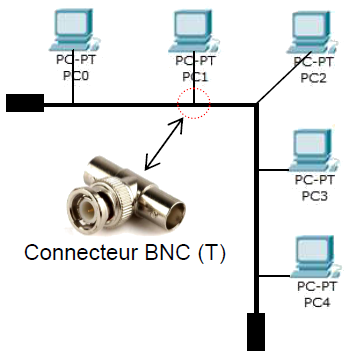
\includegraphics[width=\linewidth]{img/bus}
\end{wrapfigure}
Les machines sont reliées par un câble coaxial (le bus) et chaque ordinateur
est connecté en série sur le bus, on dit encore qu'il forme un n\oe ud.

Le câble coaxial relie les ordinateurs du réseau de manière linéaire. Il est
raccordé aux cartes réseaux par l'intermédiaire de connecteurs BNC
(Bayonet Neill-Concelman). Chaque ordinateur doit être muni d'un T et
chaque extrémité de la chaîne doit être munie d'un bouchon de terminaison
de $50\Omega$ supprimant la réverbération des signaux transmis (renvoi en sens
inverse).

Les informations envoyées à partir d'une station sont transmises sur
l'ensemble du bus à toutes les stations. Celles-ci (trames) contiennent l'adresse de destination et c'est aux stations de reconnaître les informations qui leur sont destinées.

Les stations ne peuvent dialoguer qu'à tour de rôle. Quand deux stations
émettent ensemble il y a collision, et il faut que chaque station recommence.
Cette méthode de communication est la principale caractéristique des
réseaux \textbf{Ethernet}.

}}

{\frame{
\frametitle{La topologie en étoile}

\begin{wrapfigure}[12]{r}{3.5cm}
\vspace{-7mm}
\centering 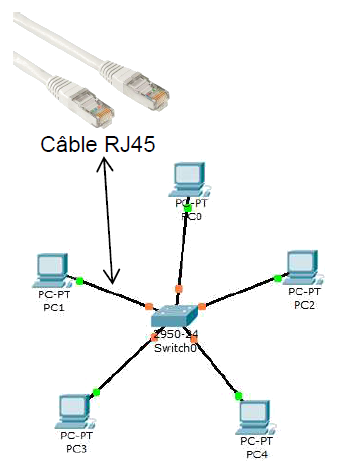
\includegraphics[width=\linewidth]{img/etoile}
\end{wrapfigure}
Notamment utilisée par les réseaux Ethernet actuels en RJ45, elle
concerne maintenant la majorité des réseaux.

Lorsque toutes les stations sont connectées à un commutateur, on
parle de topologie en étoile. Les n\oe uds du réseau sont tous reliés à
un n\oe ud central. Dans cette topologie tous les hôtes sont
interconnectés grâce à un SWITCH: sorte de multiprise pour les
câbles réseaux placés au centre de l'étoile. Les stations émettent
vers ce concentrateur qui renvoie les données vers tous les autres
ports réseaux (hub) ou uniquement au destinataire (switch). Si
les informations qui circulent sur le câblage se font de la même
manière que dans le réseau en bus, les câbles en paires torsadées
supportent un débit de 100 Mbits/s, et les switchs (les commutateurs)
peuvent diriger la trame directement à son destinataire.

Avantages: Cette topologie facilite une évolution \textbf{hiérarchisée} du matériel. On peut facilement déplacer un appareil sur le réseau. La panne d'une station (ordinateur) ne perturbe pas le fonctionnement global du réseau.

}}

{\frame{
\frametitle{La topologie en anneau}

\begin{wrapfigure}[6]{r}{3.5cm}
\vspace{-7mm}
\centering 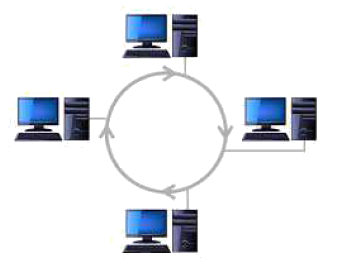
\includegraphics[width=\linewidth]{img/anneau}
\end{wrapfigure}
Dans un réseau possédant une topologie en anneau, les
ordinateurs sont situés sur une boucle et communiquent chacun à
leur tour.

Cela ressemble à un bus mais qui serait refermé sur lui-même
: le dernier n\oe ud est relié au premier.

En réalité, dans une topologie en anneau, les ordinateurs ne sont
pas reliés en boucle, mais sont reliés à un répartiteur (appelé MAU,
Multistation Access Unit).

Elle utilise la méthode d'accès à \og jeton \fg (Token ring). Les données
transitent de stations en stations en suivant l'anneau qui chaque fois
régénèrent le signal. Le jeton détermine quelle station peut émettre,
il est transféré à tour de rôle vers la station suivante.

Avantages: Le gros avantage est un taux d'utilisation de la bande passante proche de 90\%.

Inconvénients: Il est nécessaire d'interrompre le fonctionnement du réseau lors de l'adjonction d'un nouveau poste. La panne d'une station bloque toute la communication du réseau.

}}

\section{Le protocole IP}

{\frame{
\frametitle{Le protocole IP}
\begin{itemize}
 \item Protocole très répandu,
 \item Seul protocole livré de base avec toutes les stations de travail,
 \item Protocole \og léger \fg et simple,
 \item IP est réellement ouvert,
 \item IP évolue rapidement.
\end{itemize}

}}

{\frame{
\frametitle{Le protocole IP}

\begin{center}
 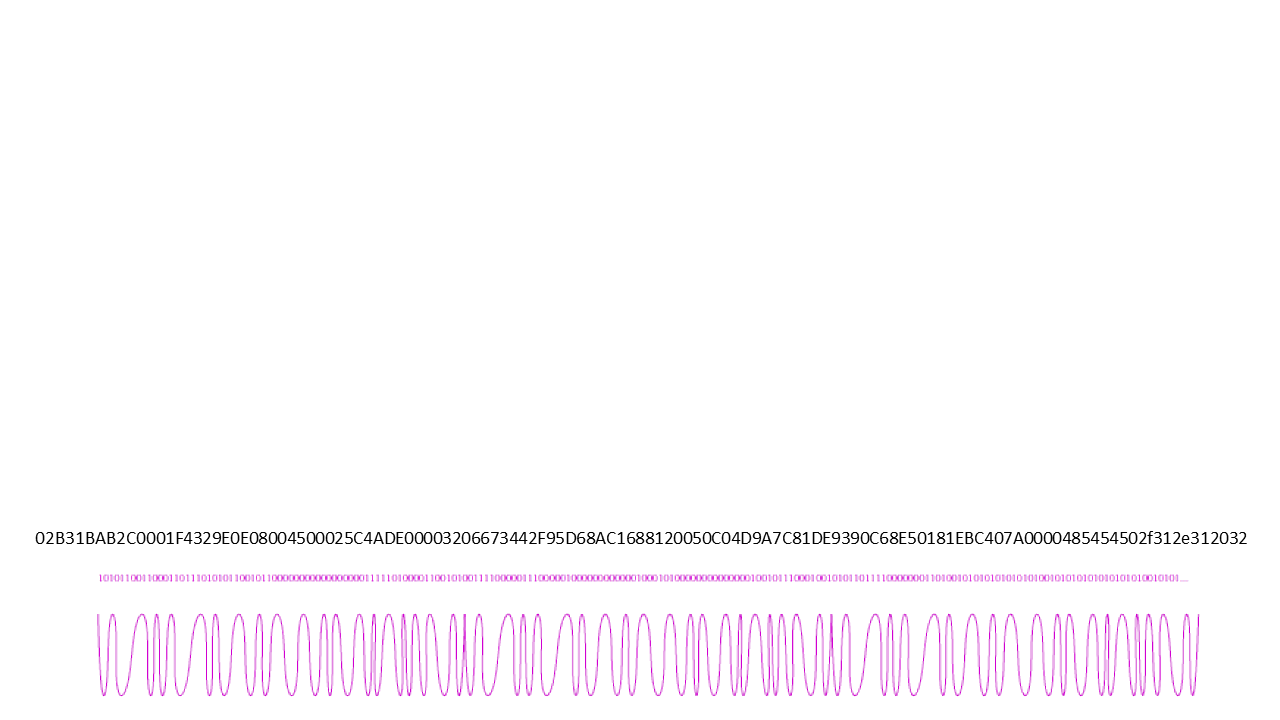
\includegraphics[width=\linewidth]{img/couches01}
\end{center}
}}

{\frame{
\frametitle{Le protocole IP}

\begin{center}
 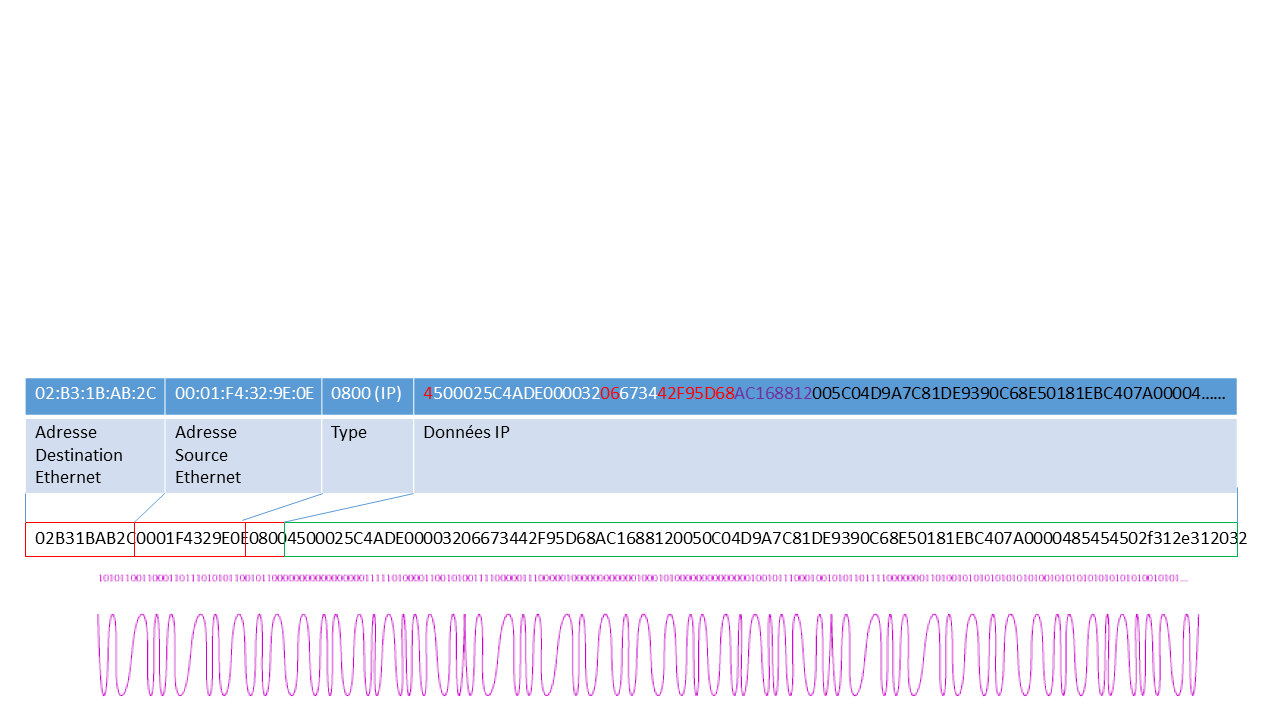
\includegraphics[width=\linewidth]{img/couches02}
\end{center}
}}

{\frame{
\frametitle{Le protocole IP}

\begin{center}
 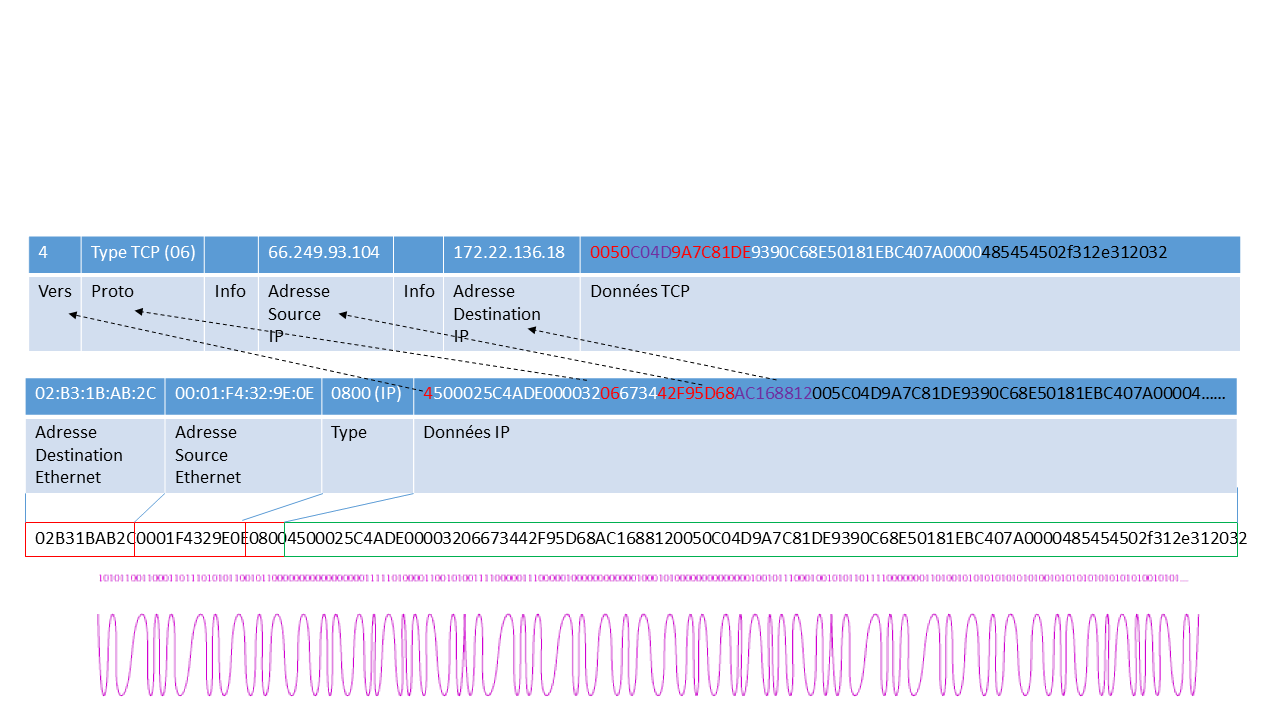
\includegraphics[width=\linewidth]{img/couches03}
\end{center}
}}

{\frame{
\frametitle{Le protocole IP}

\begin{center}
 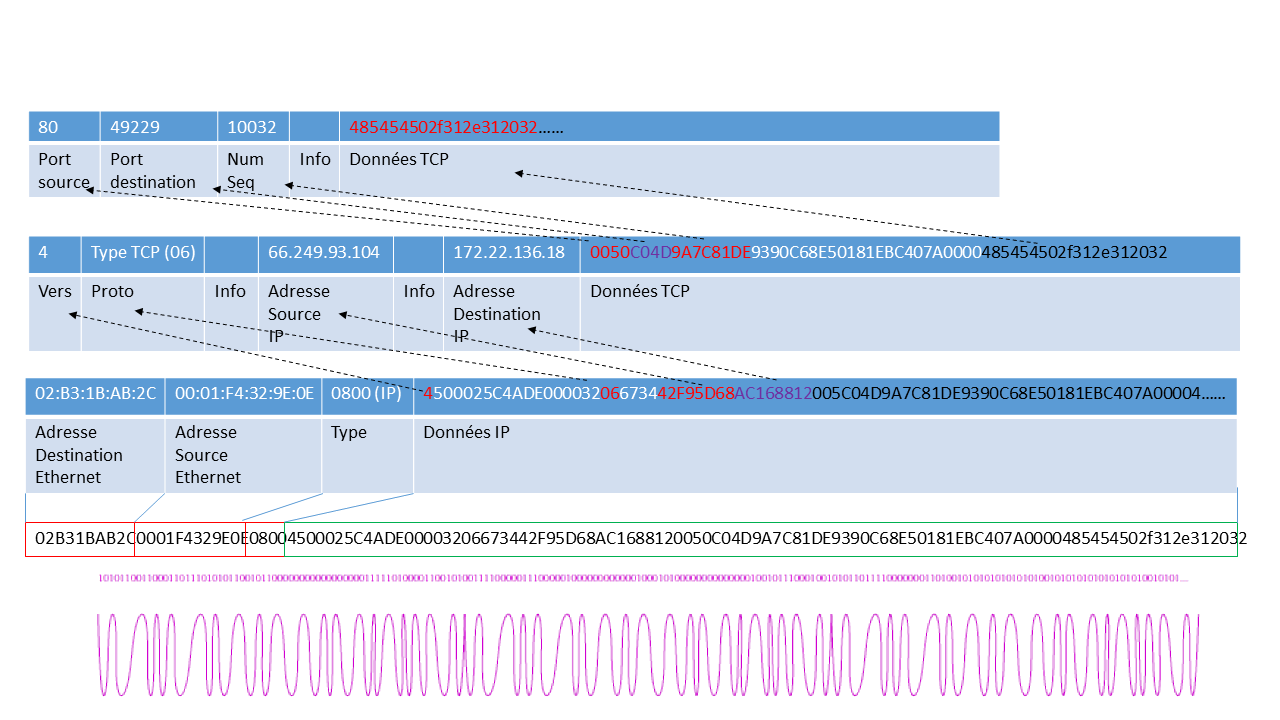
\includegraphics[width=\linewidth]{img/couches04}
\end{center}
}}

{\frame{
\frametitle{Le protocole IP}

\begin{center}
 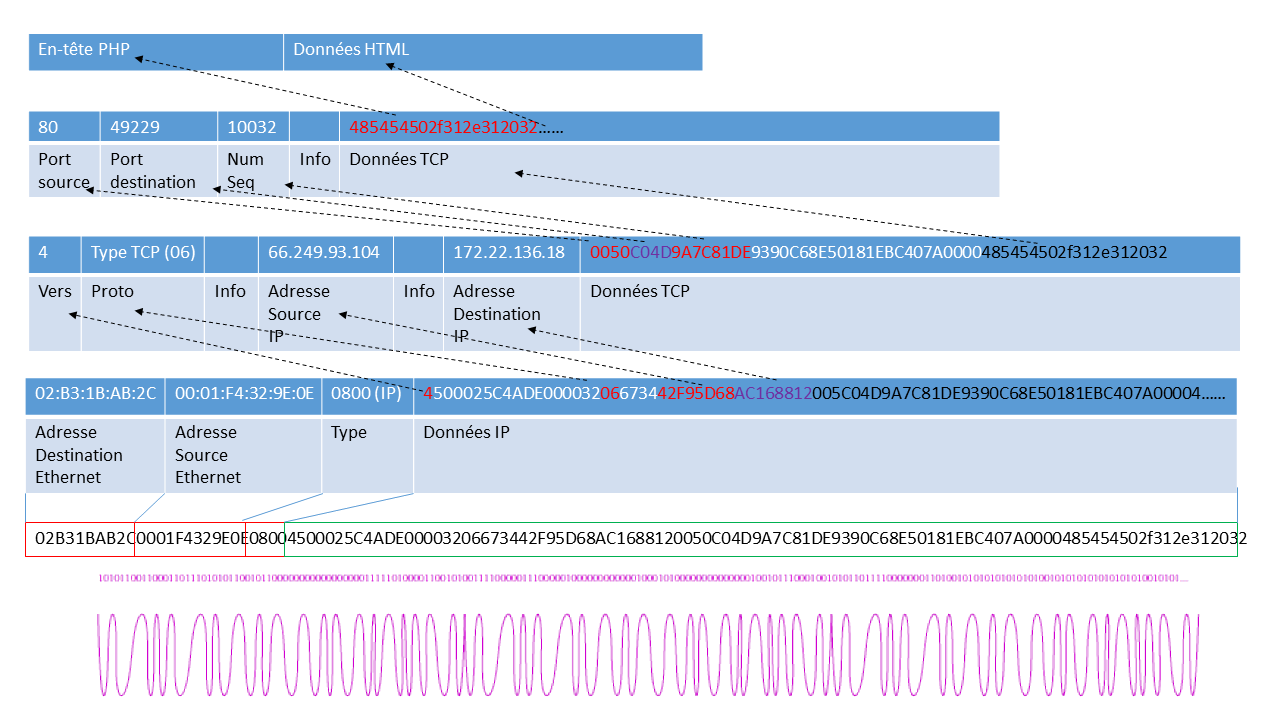
\includegraphics[width=\linewidth]{img/couches05}
\end{center}
}}

{\frame{
\frametitle{Débit}

Le débit d'un réseau mesure la quantité d'information que le réseau peut
transmettre par unité de temps :
\begin{center}
 $\text{debit}=\dfrac{\text{quantité d'information}}{\text{temps}}$
\end{center}

L'unité est par conséquent le bit par seconde, noté $b/s$ ou $b.s^{-1}$. Les réseaux actuels ayant un débit assez élevé, on utilise plus souvent des méga-bits par secondes, notés $Mb/s$.

}}


{\frame{
\frametitle{Conclusion}

\begin{savoir}
Vous êtes capables :
\begin{itemize}
 \item de déterminer l'état d'un système en fonction d'événements,
 \item de déterminer le comportement séquentiel dynamique d'un système.
\end{itemize}
\end{savoir}

\begin{prob}
Vous devez êtes capables :
 \begin{itemize}
 \item de modéliser un Système dont l'évolution est continue.
 \end{itemize}
\end{prob}
}}


\end{document}